\documentclass{article}

\usepackage[margin=1in]{geometry}
\usepackage{amsmath}
\usepackage{graphicx}
\usepackage{multicol}
\usepackage{fancyvrb}

\begin{document}
	
\title{ESOF 322 - Homework 5}
\author{Nathan Stouffer and Kevin Browder}

\maketitle
\newpage

\section*{Question 1}
\subsection*{Part A}
Problem: Create a control flowgraph for the sieve algorithm. To the left of the line numbers in the
source code clearly identify the nodes that will be used in your graph. Once you have
identified the nodes, draw the control graph. \\\\
Solution: Drawn below next to the C code.
\begin{Verbatim}[tabsize=4]
	1. /* Find all primes from 2-upper_bound using Sieve of Eratosthanes */
	2.
	3. #include
	4. typedef struct IntList {
	5.     int value;
	6.     struct IntList *next;
	7.     } *INTLIST, INTCELL;
	8. INTLIST sieve (int upper_bound ) {
	9.
	10.     INTLIST prime_list = NULL; /* list of primes found */
	11.     INTLIST cursor; /* cursor into prime list */
	12.     int candidate; /* a candidate prime number */
	13.     int is_prime; /* flag: 1=prime, 0=not prime */
	14.
	15.     /* try all numbers up to upper_bound */
	16.     for (candidate=2;
	17.
	18.         candidate <= upper_bound;
	19.         candidate++) {
	20.
	21.             is_prime = 1; /* assume candidate is prime */
	22.             for(cursor = prime_list;
	23.
	24.                 cursor;
	25.                 cursor = cursor->next) {
	26.
	27.                     if (candidate % cursor->value == 0) {
	28.
	29.                         /* candidate divisible by prime */
	30.                         /* in list, can't be prime */
	31.                         is_prime = 0;
	32.                         break; /* "for cursor" loop */
	33.                     }
	34.             }
	35.             if(is_prime) {
	36.
	37.                 /* add candidate to front of list */
	38.                 cursor = (INTLIST) malloc(sizeof(INTCELL));
	39.                 cursor->value = candidate;
	40.                 cursor->next = prime_list;
	41.                 prime_list = cursor;
	42.             }
	43.         }
	44.     return prime_list;
	45. }
\end{Verbatim}

\subsection*{Part B}
Problem: Provide a set of test cases that would give 100\% Node Coverage (NC). \\\\
Solution:\\
Test Case 1: \\
Input: 4 \\
Expected Output: [3, 2]\\
Actual Output: [3, 2]\\
$T = \{ t_1 = \{1, 2, 3, 4, 5, 6, 7, 8, 9, 10, 11, 12, 13, 14\}\}$
\subsection*{Part C}
Problem: Provide a set of test cases that would give 100\% Edge Coverage (EC). \\\\
Solution: \\
Test Case 1: \\
Input: 4 \\
Expected Output: [3, 2]\\
Actual Output: [3, 2]\\
$T = \{ t_1 = \{1, 2, 3, 4, 5, 6, 7, 8, 9, 10, 11, 12, 13, 14\}\}$
\subsection*{Part D}
Problem: Is 100\% NC or 100\% EC possible in general? Why, or why not? \\\\
Solution: 
No, it is not possible in general because there are some nodes/edges that are impossible to cover.
Example: 
\begin{Verbatim}[tabsize=4]
if(i < 0){
	if(i > 0){
		//do stuff
	}
}	
\end{Verbatim}
In this example it would be impossible to get 100\% EC or 100\% NC because once you are in first if statement there is no way to get into the second if statement. This example shows that it is not possible in general to get 100\% EC and 100\% NC.
\newpage

\section*{Question 2}

\subsection*{Part A}
Problem: Draw the execution of the calls that exhibit the YoYo problem for a runtime trace of
C3.B, and for C4.A (Draw both on the diagram below). \\\\
\begin{figure}[h]
	\centering
	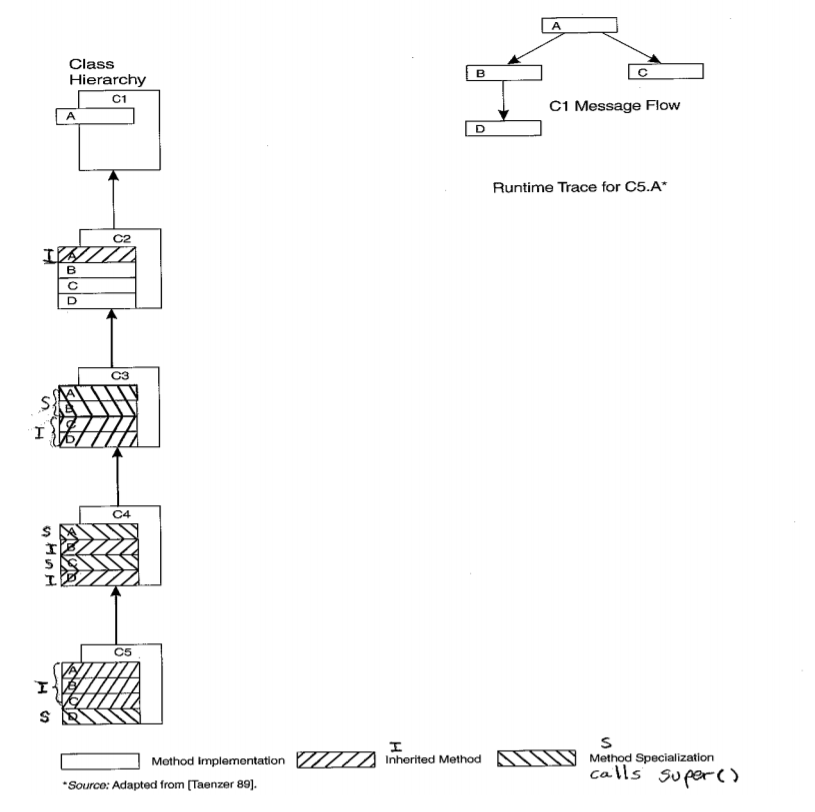
\includegraphics[width=6in]{yo-yo-diagram.png}
\end{figure}
\newpage
\subsection*{Part B}
Problem: Describe what happens when we call C1.D \\\\
Solution: An error occurs when you call C1.D. This is because of the nature of inheritance in object oriented programming. Inheritance works from the superclass down and is \textit{not} bidirectional relationship. This is what give inheritance its power, classes higher in the hierarchy do not implement methods below them. If they did there would be no point in using inheritance, it would be the same as making one big class because all the classes would share each others methods. This would also violate the dependency inversion design principle because classes high in the hierarchy would rely on classes lower in the hierarchy.

\newpage

\section*{Question 3}
Given the following program:
\begin{Verbatim}[tabsize=4]
	1. public int fibonacci (int i) { 
	2.     int fib1 = 1;    // fib(n-1)
	3.     int fib2 = 1;    // fib(n-2)
	4.     int fib = 0;
	5.     int j;

	6.     if (i <= 1) 
	7.         fib = 1;
	       else 
	8.        for (j = 1;
	9.             j < i;
	10.             j++) {
	11.            fib = fib2 + fib1;
	12.            fib2 = fib1;
	13.            fib1 = fib;
	          }
	14.    return fib;		
	   }
\end{Verbatim}
\bigskip
\noindent
Problem: Give test cases that will kill the following mutations: \\
a. Line 6: if (i $<$ 1)	\\
b. Line 6: if (i == 1)	\\
c. Line 12: fib2 = fib;	\\\\
Solution:\\
\begin{multicols}{2}
\noindent
a. normal: \\
	input = 1 \\
	return = 1 \\
	expected = 1 \\
	mutant: \\
	input = 1 \\
	return = 0 \\
	expected = 1\\
Returns not equal, mutant killed \\\\\\
b.normal: \\
input = 0 \\
return = 1 \\
expected = 1 \\
mutant: \\
input = 0 \\
return = 0 \\
expected = 1 \\
Returns not equal, mutant killed \\\\
\end{multicols}
\noindent
c.normal: \\
input = 3 \\
return = 3 \\
expected = 3 \\
mutant: \\
input = 3 \\
return = 4 \\
expected = 3 \\
Returns not equal, mutant killed \\\\

	

\end{document}